\subsection{Topología ferroviaria original}

	El primer ejemplo, ilustrado en la Figura \ref{fig:EJ1_1}, es una topología diseñada en base a dos líneas principales y tres niveles de ramificaciones. La primera ramificación, utilizando el cambio de vías Sw06, es una ramificación simple. La segunda ramificación, utilizando el cambio de vías Sw04, es una ramificación compleja al incluir el cambio de vías Sw07 a continuación. Ademas, se incluyeron los cambios de vías Sw12 y Sw13 para permitir el intercambio de formaciones entre ambas vías principales. El objetivo de este ejemplo fue comprobar el funcionamiento del RNA con una topología de múltiples ramificaciones anidadas.
	
	\begin{figure}[h]
		\centering
		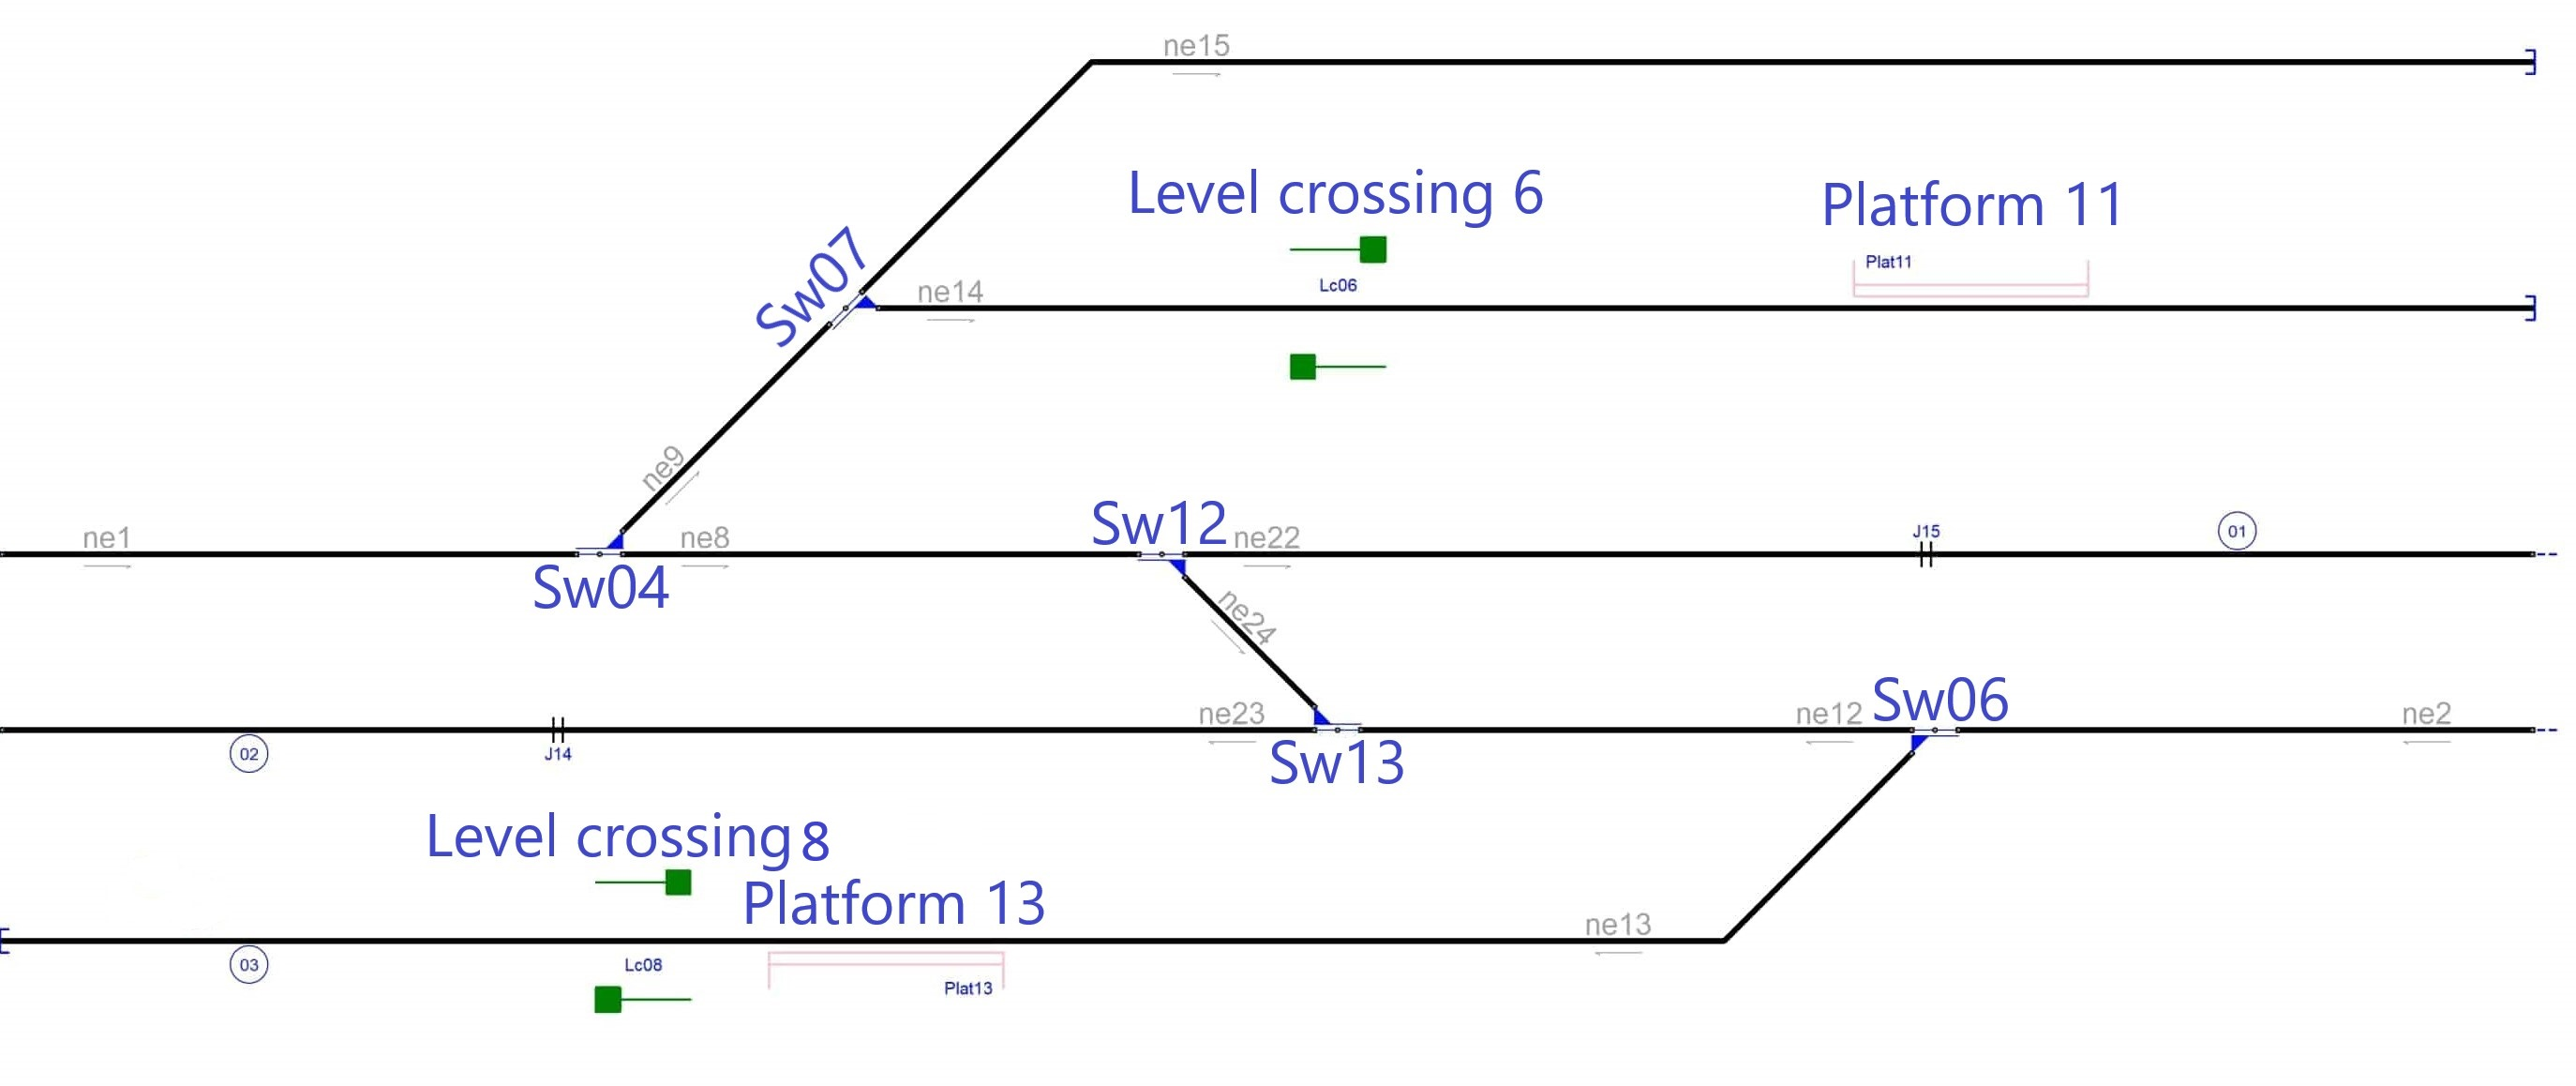
\includegraphics[width=1\textwidth]{resultados-obtenidos/ejemplo1/images/1_empty.png}
		\centering\caption{Topología ferroviaria del ejemplo 1 sin señalamiento.}
		\label{fig:EJ1_1}
	\end{figure}
	
	Para incrementar la dificultad del análisis y obtener resultados mas completos, se incluyeron finales de vías relativos y absolutos, junto con plataformas (Platorm11, Platform13) y cruces de vías (LevelCrossing06, LevelCrossing 08). La infraestructura se distribuyó de forma tal que no en todos los casos existiese espacio suficiente entre los elementos ferroviarios. Por ejemplo, entre la plataforma Platform11 y el cruce de vía LevelCrossing6 existe el espacio suficiente, en cambio entre la plataforma Platform13 y el cruce de vía LevelCrossing8 no existe tanto espacio entre ellos.